\documentclass[tikz,border=3pt]{standalone}
\usepackage[utf8]{inputenc}
\usepackage[T1]{fontenc}
\usepackage{lmodern}
\renewcommand{\familydefault}{\sfdefault}
\usepackage{sansmath}\sansmath
\usepackage{chemfig}
\usepackage{pgfplots}\pgfplotsset{compat=1.18,/pgf/number format/use comma,/pgf/number format/1000 sep={.}}
\usetikzlibrary{arrows.meta,calc,positioning,decorations.pathmorphing,patterns}
% paleta del sitio
\definecolor{nar}{HTML}{E8680C}\definecolor{narc}{HTML}{FFB35C}\definecolor{hielo}{HTML}{FFF3E8}
\definecolor{tinta}{HTML}{1D1D1F}\definecolor{gris}{HTML}{6E6E73}\definecolor{lila}{HTML}{7C5CF0}
\definecolor{azul}{HTML}{2F6FD6}\definecolor{menta}{HTML}{17A673}\definecolor{coral}{HTML}{E8342A}
\begin{document}
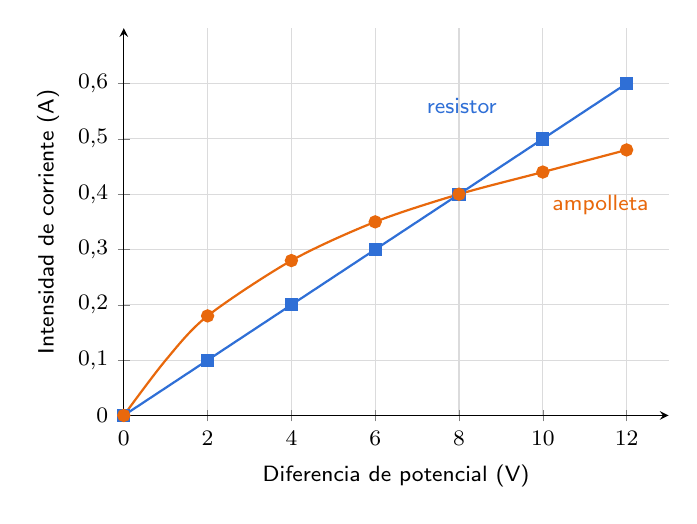
\begin{tikzpicture}[font=\footnotesize]
\begin{axis}[width=8.5cm,height=6.5cm,xmin=0,xmax=13,ymin=0,ymax=0.7,xtick={0,2,...,12},ytick={0,0.1,0.2,0.3,0.4,0.5,0.6},grid=major,grid style={gris!25},
  yticklabel style={/pgf/number format/fixed,/pgf/number format/precision=1},
  xlabel={Diferencia de potencial (V)},ylabel={Intensidad de corriente (A)},axis lines=left,every axis plot/.append style={thick}]
\addplot[azul,mark=square*,mark size=2pt] coordinates {(0,0)(2,0.1)(4,0.2)(6,0.3)(8,0.4)(10,0.5)(12,0.6)};
\addplot[nar,smooth] coordinates {(0,0)(1,0.1)(2,0.18)(4,0.28)(6,0.35)(8,0.4)(10,0.44)(12,0.48)};
\addplot[nar,only marks,mark=*,mark size=2pt] coordinates {(0,0)(2,0.18)(4,0.28)(6,0.35)(8,0.4)(10,0.44)(12,0.48)};
\node[text=azul,anchor=west] at (axis cs:7.0,0.56) {resistor};
\node[text=nar,anchor=west] at (axis cs:10.0,0.38) {ampolleta};
\end{axis}
\end{tikzpicture}
\end{document}
